% !TEX root = ../main.tex
\section{Evaluation Protocol and Metrics}
\label{app:evaluation}

A trained flow is evaluated in three passes that answer different questions
(\cref{tab:evaluation-passes}). Two of them use the truth to pair drawn and injected sources,
and are therefore descriptive; only the validation pass, which never sees the truth, tests
calibration. A Gaussian Fisher forecast and a reference \ac{mcmc} (\cref{app:mcmc}) give
widths to compare against. Results are in \cref{app:results}.

\begin{table}[h]
  \centering
  \caption{The three evaluation passes.}
  \label{tab:evaluation-passes}
  \small
  \begin{tabular}{@{}l>{\raggedright\arraybackslash}p{0.27\textwidth}r>{\raggedright\arraybackslash}p{0.36\textwidth}@{}}
    \toprule
    Pass & Injections & Draws & Use \\
    \midrule
    Eval & \EvaluationQuantilesWord{} fixed windows at quantiles of the window \acs{snr}
         & \EvaluationPosterior & corner plots; comparison with Fisher and \acs{mcmc} \\
    Scorecard & the same plus \EvaluationRandom{} prior windows (\EvaluationWindows{} in all)
         & \EvaluationDraws & widths, detection, offsets, coverage per \acs{snr} band;
           descriptive, uses the truth \\
    Validation & \EvaluationValidation{} prior windows from a separate key
         & \EvaluationValidationDraws & rank tests and proper scores; never sees the truth \\
    \bottomrule
  \end{tabular}
\end{table}

\subsection{Weights and Sampler}
\label{app:evaluation-weights}

Every pass evaluates the schedule-free average of the weights, the sequence $\bar\vartheta$ of
\citet{defazio2024road} whose convergence the method guarantees (\cref{app:training}); the
interpolated weights at which gradients are taken are never reported. The default flow
predicts $x_1$ (\cref{app:fm}), and the sampler takes \EvaluationOdeSteps{} midpoint steps
toward the predicted $x_1$, each exact if the prediction were constant along the step; a
velocity-predicting flow takes fourth-order Runge--Kutta steps instead. The base draws are
prior draws in flow coordinates (\cref{app:chart}), so a flow that ignored the data would
return the prior. A run is evaluated in the precision it was trained in.

\subsection{Eval Injections}
\label{app:evaluation-injections}

From \EvaluationCandidates{} candidate windows drawn from the prior, each a centre frequency
$\fw$ with \EvaluationNSources{} sources (\cref{app:priors}), the eval injections are the
candidates at the quantiles \EvaluationQuantiles{} of the window \ac{snr}, that of the summed
signal. They span window \acp{snr} \EvaluationNarrowSnrLo--\EvaluationNarrowSnrHi{} in the
narrow band and \EvaluationFullSnrLo--\EvaluationFullSnrHi{} in the full band, and source
\acp{snr} \EvaluationSourceSnrLo--\EvaluationSourceSnrHi. Injections and noise are fixed by the
run's seed and band, so every checkpoint and every run on the same band sees the same data,
and so do the reference chains. Selecting by \ac{snr} spreads the injections from faint to loud
windows, which a handful of prior draws would not; it also makes them a conditional sample,
for inspection and never for calibration.

\subsection{Relabelling Draws to the Truth}
\label{app:evaluation-matching}

The flow emits its sources in slots sorted loudest first (\cref{app:network}). Sorting removes
the exact permutation symmetry of the likelihood but not the label switching it causes
\citep{stephens2000dealing,jasra2005markov,buscicchio2019label}: two sources of nearly equal
\ac{snr} swap slots from draw to draw, because their \acp{snr} are themselves uncertain. For
display and for the scorecard, each draw $\theta_{1:S}$ is relabelled to the truth
$\theta^\star_{1:S}$ by the permutation
\begin{gather}
  \hat\sigma = \operatorname*{arg\,min}_{\sigma\in\mathfrak S_S}
  \sum_{s=1}^{S}\bigl\|\mathbf m(\theta_{\sigma(s)}) - \mathbf m(\theta^\star_s)\bigr\|^2,
  \label{eq:evaluation-matching}\\
  \mathbf m(\theta) = \Bigl(\frac{f_0}{f_+ - f_-},\ \log_{10}\Amp,\ \hat n(\alpha,\delta)\Bigr),
  \nonumber
\end{gather}
found exhaustively over the $S! = \EvaluationPermutations$ permutations, with $(f_-, f_+)$ the
window's frequency range and $\hat n$ the unit sky vector. The features tell sources apart: the
best-measured parameter in units of the window, the amplitude that orders them, and the sky
with no wrap in longitude. The orientation angles are left out, since their exact symmetries
(\cref{eq:psi-phi-symmetry}) would make the cost multimodal.

The relabelling uses the truth, so a posterior too wide to separate two sources is sorted back
onto them and looks better resolved and better calibrated than it is. Everything computed after
it is descriptive.

\subsection{Scorecard}
\label{app:evaluation-scorecard}

The scorecard adds \EvaluationRandom{} unpicked candidates, plain prior draws, to the eval
injections, for \EvaluationWindows{} windows and \EvaluationWindowSources{} sources. After the
relabelling, each source gets the quantities of \cref{tab:evaluation-scorecard}, with $f_0$ in
frequency bins of $1/\Tobs$. Sources are grouped by their true \ac{snr} in bands
$<\EvaluationBandOne$, \EvaluationBandOne--\EvaluationBandTwo,
\EvaluationBandTwo--\EvaluationBandThree{} and $\ge\EvaluationBandThree$: the source \acp{snr}
run from \EvaluationSnrLo{} to \EvaluationSnrHi{} (\cref{app:priors}), so the ideal width runs
from \EvaluationIdealLo{} to \num{\EvaluationIdealHi} bins and is only meaningful per band.

\begin{table}[h]
  \centering
  \caption{Scorecard quantities per source, on the relabelled draws.}
  \label{tab:evaluation-scorecard}
  \small
  \begin{tabular}{@{}l>{\raggedright\arraybackslash}p{0.48\textwidth}l@{}}
    \toprule
    Quantity & Definition & Per band \\
    \midrule
    Width $w$ & $1.4826\,\MAD(f_0)$; the standard deviation for a Gaussian, robust to stray draws
      & median over found \\
    Width ratio & $w/w^\star$, with $w^\star$ of \cref{eq:evaluation-ideal-width} at the source's \acs{snr}
      & median over found \\
    Found & $w < \EvaluationFound\bins$: the frequency is pinned to the bin spacing
      & fraction \\
    Offset & median of $f_0$ minus the truth & median over found \\
    Rank & fraction of draws below the true $f_0$ & mean \\
    Coverage & truth inside the central \qty{68}{\percent} and \qty{95}{\percent} intervals & mean \\
    \bottomrule
  \end{tabular}
\end{table}

The coverage and rank columns show where the flow is wide or biased, but they are not a
calibration test: the relabelling uses the truth, the bands are cut on the true \ac{snr}, and the
eval injections are selected by \ac{snr}.

\paragraph{The ideal width.}
For a sinusoid of \ac{snr} $\snr$ observed for $\Tobs$ in stationary noise, with the time origin
at the centre of the observation, the Fisher matrix in angular frequency and phase is diagonal,
$\Gamma_{\omega\omega} = \snr^2\Tobs^2/12$ and $\Gamma_{\phi\phi} = \snr^2$, and the
amplitude decouples. The frequency width is then
\begin{equation}
  w^\star = \frac{\sqrt{12}}{2\pi\,\snr\,\Tobs}\,\Tobs = \frac{\sqrt3}{\pi\,\snr}\bins.
  \label{eq:evaluation-ideal-width}
\end{equation}
It is a yardstick, not a bound. Correlations with the chirp, the orbital Doppler shift, the sky
and the orientation widen the real frequency width, and one correlation is large by
construction: $f_0$ is the frequency at the start of the observation (\cref{app:forward-model}),
so once the chirp is measured, the quadratic phase term is fitted about one end of the interval
and the marginal width of $f_0$ grows by a factor of \EvaluationStartFactor{} over the centred
one. \Cref{fig:evaluation-fisher-width} bears this out. Over the \EvaluationSourcesBoth{} eval
sources of the two bands, the Fisher $f_0$ width is never below $w^\star$ and is a median
\EvaluationFisherRatioMedian{} times it (\EvaluationFisherRatioLo--\EvaluationFisherRatioHi).
In the narrow band, where the chirp is barely measured, the median is
\EvaluationFisherRatioNarrow{} (at most \EvaluationFisherRatioNarrowHi); in the full band it is
\EvaluationFisherRatioFull, and loud high-frequency sources sit near the factor
\EvaluationStartFactor. A full-band width ratio well above one is therefore not by itself a
failure of the flow; the Fisher width is the sharper reference there.

\begin{figure}[!htbp]
  \centering
  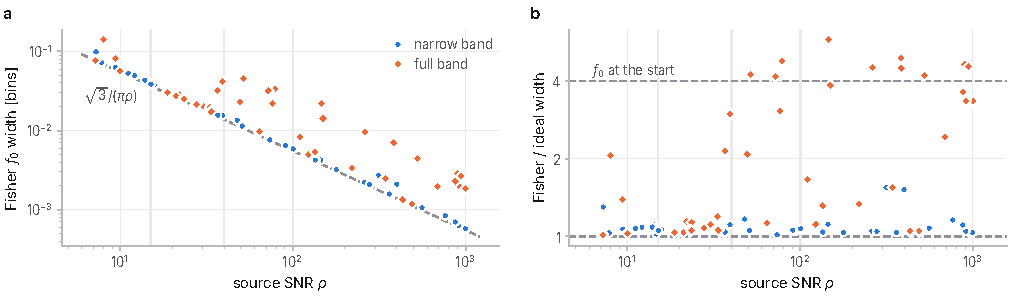
\includegraphics[width=\textwidth]{figures/fisher-width.pdf}
  \caption{The ideal width is a floor, not a forecast. (a) Fisher-forecast $f_0$ width of the
  \EvaluationSourcesBoth{} eval sources against their \ac{snr}, with the ideal width
  $\sqrt3/(\pi\snr)$ of \cref{eq:evaluation-ideal-width} (dashed). (b) Their ratio. Narrow-band
  sources stay within a factor \EvaluationFisherRatioNarrowHi{} of the ideal; full-band sources,
  whose chirp is measured, reach the factor \EvaluationStartFactor{} that a start-of-observation
  $f_0$ costs (upper dashed line). Vertical lines mark the scorecard's \ac{snr} bands.}
  \label{fig:evaluation-fisher-width}
\end{figure}

\subsection{Calibration Without the Truth}
\label{app:evaluation-validation}

The validation pass draws \EvaluationValidation{} injections, each with its own $\fw$, sources
and noise from the prior, and $M = \EvaluationValidationDraws$ flow draws on each. If the flow is
the exact posterior, the truth is exchangeable with the draws, so the rank of any scalar test
quantity $g$, the number of draws with $g(\theta_m) < g(\theta^\star)$ (ties broken at random),
is uniform on $\{0,\dots,M\}$ \citep{talts2018validating}.

The same $g$ must be applied to the truth and to every draw, without seeing the truth. Slots are
therefore defined by each parameter set's own \ac{snr}: the truth and each draw are sorted,
independently, by the \acp{snr} of their own sources. This is a fixed function of the
parameters, so the ranks stay uniform under an exact posterior, unlike those after
\cref{eq:evaluation-matching}. Strata follow the same rule: a source is binned in the
scorecard's \ac{snr} bands by $\hat\snr$, the median own \ac{snr} of the draws in its slot, and the
window quantities by the draws' median total \ac{snr}. Binning by the true \ac{snr} would condition on
the truth, and the ranks need not be uniform within such a bin even for an exact posterior.

\Cref{tab:evaluation-tests} lists the test quantities and scores. Ranks of the parameters alone
cannot catch every error: the prior, taken as a posterior, passes them, and so does \ac{tarp}
with a prior reference point. Quantities that depend on the data, the overlap and the
log-likelihood, catch it \citep{modrak2023simulation}, as the power study below confirms
(\cref{tab:evaluation-power}). The likelihood enters only as a test
quantity on draws the flow has already made, never in inference.

\begin{table*}[t]
  \centering
  \caption{Validation test quantities (rank tests, top) and scores (bottom). ``Slot'' is per
  source slot, ``window'' is over all \EvaluationJointDim{} coordinates of a window.}
  \label{tab:evaluation-tests}
  \small
  \begin{tabular}{@{}>{\raggedright\arraybackslash}p{0.33\textwidth}l>{\raggedright\arraybackslash}p{0.47\textwidth}@{}}
    \toprule
    Quantity & Level & What it catches \\
    \midrule
    The eight flow coordinates (\cref{eq:chart}) & slot & bias or wrong width in one coordinate \\
    Sum and difference of the $f_0$ and $\Mc$ coordinates & slot & errors along their correlation \\
    Radii $|z_\pm|$ of the amplitude--phase coordinates & slot & amplitude errors, whatever the phase \\
    Overlap $\inner{d}{h_s}/\inner{h_s}{h_s}^{1/2}$ (\cref{eq:inner}) & slot & draws that do not fit the data; a prior-like posterior \\
    Own \acs{snr} of the source & slot & a bias toward loud or faint sources \\
    \acs{tarp} distance to a prior reference point \citep{lemos2023sampling} & slot, window & a joint error in coordinate space \\
    Average-rank and band-depth pre-ranks \citep{thorarinsdottir2016assessing} & slot, window & dependence errors that every marginal passes \\
    Log-likelihood (\cref{eq:loglik}) & window & a window that does not fit the data as a whole \\
    \midrule
    Energy score, \cref{eq:evaluation-energy} & slot, window & calibration and sharpness together \\
    \acs{crps} (the one-dimensional energy score) & coordinate & the same, per coordinate \\
    Width over the ideal width at $\hat\snr$ & slot & sharpness against \cref{eq:evaluation-ideal-width} \\
    \bottomrule
  \end{tabular}
\end{table*}

\paragraph{Uniformity test.}
For each quantity, stratum and slot, the ranks are tested with the graphical \ac{ecdf} test of
\citet{sailynoja2022graphical}. With $N$ ranks on $k = \EvaluationRankValues$ values, the
statistic $\gamma$ is twice the smallest binomial tail probability of the rank \ac{ecdf} at
$z_i = i/k$, $i = 1,\dots,k-1$. Its $p$-value comes from \EvaluationGammaSims{} simulated sets of
$N$ uniform ranks, which also give a simultaneous \qty{\EvaluationBandLevel}{\percent} band for the \ac{ecdf}
minus $z$; a $\chi^2$ test on a histogram depends on the binning and has no such band. Each cell
reports the $p$-value, the mean rank over $M$ minus one half (positive when the truth sits above
the draws), and the share of ranks in the middle half: above one half the posterior is too
wide, below it too narrow.

\paragraph{Scores.}
Uniform ranks say nothing about sharpness, since the prior is calibrated. The pass therefore
also reports strictly proper scores \citep{gneiting2007strictly,gneiting2007probabilistic},
which reward calibration and sharpness together, chiefly the fair energy score in flow
coordinates,
\begin{equation}
  \mathrm{ES} = \frac1M\sum_{m}\|x_m - x^\star\|
  - \frac{\sum_{m\ne m'}\|x_m - x_{m'}\|}{2M(M-1)},
  \label{eq:evaluation-energy}
\end{equation}
per slot in eight dimensions, per window in \EvaluationJointDim, and per coordinate, where it
is the \ac{crps}. Scores are medians per stratum, for comparing runs on the same injections, not
tests by themselves.

\paragraph{Size and power.}
The tests are run on a toy whose posterior is known and drawn exactly: each slot is a
linear-Gaussian model in its eight coordinates, and the test quantities, data-space ones
included, are computed on its data unchanged. Of \EvaluationPowerInjections{} injections with
\EvaluationPowerDraws{} draws each, split into chunks of \EvaluationPowerChunk, a test's rate is
the share of chunks (and slots, for per-slot tests) in which it rejects at
\qty{\EvaluationPowerAlpha}{\percent}. Each error is injected into the draws about their own
mean and standard deviation, and an energy score counts as a detection when it is worse than on
the exact draws in a one-sided paired Wilcoxon test. Under the null the rank tests hold their
size (\cref{tab:evaluation-power}). A phase or sky taken from the prior, or coordinates shuffled
across draws, leave every one-dimensional marginal exact and pass the coordinate ranks; the
overlap, the log-likelihood and the energy score catch all three, and a \qty{10}{\percent}
admixture of prior draws as well. Width errors reach the coordinate ranks only in part and the overlap
and log-likelihood fully; an $f_0$ shift is caught by the rank of $f_0$ itself and by the
log-likelihood.

\begin{table}[t]
  \centering
  \caption{Rejection rates of the validation tests on the exact-posterior toy, per error injected
  into the draws. Coordinate ranks give the range over the eight flow coordinates; overlap and own
  \acs{snr} are per slot, the log-likelihood and energy score per window. A score has no null
  distribution of its own, so its null rate is undefined.}
  \label{tab:evaluation-power}
  \small
  \begin{tabular}{@{}lccccc@{}}
    \toprule
    & & \multicolumn{3}{c}{Data-space ranks} & \\
    \cmidrule(lr){3-5}
    Injected error & Coordinate ranks & Overlap & Own \acs{snr} & Log-likelihood & Energy score \\
    \midrule
    None & \EvaluationPowerNullCoord & \EvaluationPowerNullOverlap & \EvaluationPowerNullSnr & \EvaluationPowerNullLike & \EvaluationPowerNullEnergy \\
    $z_+$ phase from the prior & \EvaluationPowerPhaseCoord & \EvaluationPowerPhaseOverlap & \EvaluationPowerPhaseSnr & \EvaluationPowerPhaseLike & \EvaluationPowerPhaseEnergy \\
    Sky from the prior & \EvaluationPowerSkyCoord & \EvaluationPowerSkyOverlap & \EvaluationPowerSkySnr & \EvaluationPowerSkyLike & \EvaluationPowerSkyEnergy \\
    Coordinates shuffled across draws & \EvaluationPowerShuffleCoord & \EvaluationPowerShuffleOverlap & \EvaluationPowerShuffleSnr & \EvaluationPowerShuffleLike & \EvaluationPowerShuffleEnergy \\
    \qty{10}{\percent} prior draws & \EvaluationPowerMixedCoord & \EvaluationPowerMixedOverlap & \EvaluationPowerMixedSnr & \EvaluationPowerMixedLike & \EvaluationPowerMixedEnergy \\
    Width $\times0.8$ & \EvaluationPowerNarrowCoord & \EvaluationPowerNarrowOverlap & \EvaluationPowerNarrowSnr & \EvaluationPowerNarrowLike & \EvaluationPowerNarrowEnergy \\
    Width $\times1.25$ & \EvaluationPowerWideCoord & \EvaluationPowerWideOverlap & \EvaluationPowerWideSnr & \EvaluationPowerWideLike & \EvaluationPowerWideEnergy \\
    $f_0$ shifted by $0.5\sigma$ & \EvaluationPowerShiftCoord & \EvaluationPowerShiftOverlap & \EvaluationPowerShiftSnr & \EvaluationPowerShiftLike & \EvaluationPowerShiftEnergy \\
    \bottomrule
  \end{tabular}
\end{table}

\subsection{Fisher Forecast}
\label{app:evaluation-fisher}

Each eval injection gets a Gaussian forecast centred at the truth $\theta^\star$, in the
\EvaluationJointDim{} physical parameters of its sources, with precision
\begin{equation}
  \Gamma = \frac1{N_{\rm F}}\sum_{r=1}^{N_{\rm F}}\nabla^2_\theta\bigl[-\log L(\theta; d_r)\bigr]_{\theta^\star}
  + \Lambda,
  \qquad N_{\rm F} = \EvaluationFisherDraws,
  \label{eq:evaluation-fisher}
\end{equation}
with $\log L$ from \cref{eq:loglik} and $d_r$ independent noise realisations around the
injection's signal. The noise average of the Hessian at the truth is the Fisher matrix
\citep{cutler1994gravitational,vallisneri2008use}. The prior term $\Lambda$, the inverse
covariance of the candidates' parameters, is a Gaussian stand-in for the prior that keeps poorly
measured directions at the prior's width rather than infinite.

The forecast is drawn in $q$, the parameters with $\log\Mc$ in place of $\Mc$, so the chirp
mass stays positive ($\Gamma$ and $\Lambda$ pick up the Jacobian
$J = \mathrm{diag}(1, \Mc^\star, 1,\dots)$ on both sides). In physical units the diagonal of
$\Gamma$ spans a median of \EvaluationFisherDecades{} decades
(\EvaluationFisherDecadesLo--\EvaluationFisherDecadesHi{} per injection), so both matrices are
rescaled to unit diagonal, $\tilde\Gamma = D^{-1}\Gamma D^{-1}$ with
$D = \mathrm{diag}\sqrt{|\Gamma_{ii}|}$. With $\tilde\Gamma = \sum_k w_k v_k v_k^{\T}$, each
eigenvalue is floored at the prior precision along its eigenvector:
\begin{equation}
  q = q^\star + D^{-1}\sum_k \frac{\xi_k\,v_k}{\sqrt{\max(w_k,\,v_k^{\T}\tilde\Lambda v_k)}},
  \quad \xi_k \sim \Normal(0,1).
  \label{eq:evaluation-fisher-draws}
\end{equation}

The floor is needed because a finite noise average leaves part of the data-dependent term of the
Hessian, which along a barely constrained direction can outweigh the signal term. The averaged
chirp-mass diagonal is not positive for \EvaluationMcNegative{} of the \EvaluationSourcesBoth{}
eval sources, in \EvaluationMcNegativeInjections{} of the \EvaluationFisherInjections{}
injections. The floor binds only where the averaged Hessian is negative along an eigenvector,
for at most \EvaluationFlooredMax{} eigenvalues, in \EvaluationFlooredInjections{} injections.

The forecast is a reference width, not a posterior: it is unimodal, so it misses the exact
symmetries of \cref{eq:psi-phi-symmetry}; it is Gaussian, so it cannot follow the curved
amplitude--inclination degeneracy; and along a parameter the data barely constrain it shows the
prior's width centred on the truth. That is the chirp mass in the narrow band: at its top
frequency, \qty{\EvaluationNarrowFzeroTop}{\milli\hertz}, the heaviest chirp mass of the prior,
\qty{\EvaluationMcTop}{\solarmass}, drifts by \EvaluationChirpDrift{} bins over the mission, while with
$f_0$ free a drift is resolved only to about $\EvaluationDriftResolution/\snr$ bins.
\Cref{app:mcmc-fisher} tests the forecast against the joint chains.

\subsection{Comparison With the Reference \acs{mcmc}}
\label{app:evaluation-mcmc}

The reference \ac{mcmc} (\cref{app:mcmc}) runs on the same eval injections with the same noise;
corner plots overlay its draws and the Fisher draws on the relabelled flow draws, with
$(\psi,\phi_0)$ folded onto the copy nearest the truth. Orientation widths are compared through
the phases $\phi_0 \pm 2\psi$ of the two amplitude--phase coordinates: the data pin the one whose
amplitude dominates, while $\phi_0$ alone inherits the spread of $\psi$. The \ac{mcmc} is an
evaluation reference only; no likelihood or chain output enters training or the flow's draws.

\textcolor{red}{TODO(new runs): scorecard and validation tables for narrow-B and full-B, in \cref{app:results}.}
